\documentclass{article}
\usepackage[margin=1.5in]{geometry}

\usepackage{graphicx, multirow}

\usepackage{amsmath, amssymb, amsthm, bm}
\mathchardef\mhyphen="2D
\DeclareMathOperator*{\argmax}{argmax}
\newcommand{\indep}{\perp\!\!\!\perp}
\newcommand{\nindep}{\not\!\indep}
\newcommand*\diff{\mathop{}\!\mathrm{d}}
\newcommand*\Diff[1]{\mathop{}\!\mathrm{d^#1}}

\usepackage[parfill]{parskip}
\setlength\parindent{0pt}

\usepackage{hyperref}
\hypersetup{
    colorlinks,
    citecolor=black,
    filecolor=black,
    linkcolor=black,
    urlcolor=black
}

\includeonly{
    2-probability/2-probability,
    3-discrete-generative-models/3-discrete-generative-models,
    % 4-gaussian-models/4-gaussian-models,
}

\title{Rough solutions to\\\textit{Machine Learning: A Probabilistic Perspective}\\by Kevin Murphy}
\author{Alfred Wong}
\date{\vspace{-\baselineskip}}
\begin{document}
\maketitle
\pagebreak
\tableofcontents
\pagebreak

\section{Introduction}
These exercises offer a practical introduction to some machine learning concepts using KNN and MNIST. Will revisit this later as I'm currently more concerned with the theoretical stuff.
\subsection{KNN classifier on shuffled MNIST data}
Takes about 19:47 minutes to run on my computer and achieves a test set accuracy of 96.61\%.
\subsection{Approximate KNN classifiers}
Cool idea. [TODO]
\subsection{CV for KNN}
5-fold leave one out cross validation predicts 96.94\% accuracy. Takes 1:30:45 hours to run in total.
\section{Probability}
\subsection{Boys \& girls}
\textit{(Source: Minka). My neighbour has two children. Suppose I ask him whether he has any boys, and he says yes. What is the probability that one child is a girl?}

\begin{align*}
\mathbb{P}(BG \lor GB | BB \lor BG \lor GB) &= \frac{\mathbb{P}((BG \lor GB) \land (BB \lor BG \lor GB))}{\mathbb{P}(BB \lor BG \lor GB)} \\
&= \frac{\mathbb{P}(BG \lor GB)}{\mathbb{P}(BB \lor BG \lor GB)} \\
&= \frac{2}{3}
\end{align*}

This result is somewhat interesting because you might expect that knowing your neighbour has any boys would decrease the likelihood of having one girl, which is 1/2 a priori. However, we can see from the above that this works because the conditionining cuts out the GG case, where there is not exactly one girl.

\textit{Suppose instead that I happen to see one of his children run by, and it is a boy. What is the probability that the other child is a girl?}

Without loss of generality, we can assume that we saw child 1. Thus
\begin{gather*}
\mathbb{P}(BG | BB \lor BG) = \frac{\mathbb{P}(BG \land (BB \lor BG))}{\mathbb{P}(BB \lor BG)} = \frac{\mathbb{P}(BG)}{\mathbb{P}(BB \lor BG)} = \frac{1}{2}
\end{gather*}

In this case, observing one child does not have any bearing on the gender of the other, as expected. This is different from the previous problem because there we were given information that affected both children. As suggested by the heading, subtle differences in phrasing can lead to very different probabilities.

\textit{(Bonus question). Along the theme of genders of children, another somewhat interesting problem arises when we are given that one of the children is a boy, born on a Tuesday. Now, what is the probability of both children being boys?}

\begin{table}[!h]
\centering
    \begin{tabular}{cc|cccc}
    &   & \multicolumn{2}{c}{B}   & \multicolumn{2}{c}{G} \\
    &   & T          & N          & T         & N         \\ \hline
\multirow{2}{*}{B} & T & \textbf{1} & \textbf{6} & 1         & 6         \\
    & N & \textbf{6} & $\ast$     & $\ast$    & $\ast$    \\
\multirow{2}{*}{G} & T & 1          & $\ast$     & $\ast$    & $\ast$    \\
    & N & 6          & $\ast$     & $\ast$    & $\ast$   
\end{tabular}
\end{table}

13/27.

\subsection{Legal reasoning}
\textit{(Source: Peter Lee). Suppose a crime has been committed. Blood is found at the scene for which there is no innocent explanation. It is of a type which is present in 1\% of the population.}

\textit{The prosecutor claims: ``There is a 1\% chance that the defendant would have the crime blood type if he were innocent. Thus there is a 99\% chance that he is guilty."}

\textit{The defender claims: ``The crime occurred in a city of 800,000 people. The blood type would be found in approximately 8000 people. The evidence has provided a probability of just 1 in 8000 that the defendant is guilty, and thus has no relevance."}

Denote $A$ as having the crime blood type and $B$ as being innocent. The prosecutor's argument has two flaws. First, it assumes that $\mathbb{P}(A|B) = 1\% = \mathbb{P}(A)$, which is not generally true, although it is likely. Worse, it then asserts that $\mathbb{P}(A|B) + \mathbb{P}(\neg B|A) = 1$, which is just clearly not true in general.

For the defender's argument, assuming that the blood type test is 100\% sensitive, i.e. $\mathbb{P}(A|\neg B) = 1$, then it is certainly true that $\mathbb{P}(\neg B|A) = \mathbb{P}(\neg B)/\mathbb{P}(A)$. So, if the defendant was randomly pulled off the streets, and this was the only incriminating evidence available, it is likely that the case would be insufficient for a conviction. This is a good thing.

However, the fact that the defendant is under trial probably means that they were not randomly selected in the first place. Denoting $D$ as being placed under trial, we actually want to know $\mathbb{P}(\neg B|A \land D) = \mathbb{P}(\neg B|D)/\mathbb{P}(A|D)$. Far from being `irrelevant', the evidence has the effect of increasing our prior suspicion of involvement by a factor of 100, assuming that $\mathbb{P}(A|D) = \mathbb{P}(A)$. The defender's fallacy lies in the assertion that this prior suspicion is only 1/800,000.

\subsection{Variance of a sum}
Suppose $X$ and $Y$ are random variables with means $\mu_X$ and $\mu_Y$, variances $\sigma_X^2$ and $\sigma_Y^2$, and covariance $\sigma_{XY}$. Let $Z = X + Y$. Then
\begin{align*}
\sigma_Z^2 &= \mathbb{E}[Z^2] - \mu_Z^2\\
&= \mathbb{E}[X^2 + Y^2 + 2XY] - (\mu_X^2 + \mu_Y^2 + 2\mu_X\mu_Y)\\
&= \mathbb{E}[X^2] - \mu_X^2 + \mathbb{E}[Y^2] - \mu_Y^2 + 2(\mathbb{E}[XY] - \mu_X\mu_Y)\\
&= \sigma_X^2 + \sigma_Y^2 + 2\sigma_{XY}.
\end{align*}

Since $|\sigma_{XY}| \leq \sigma_X\sigma_Y$, this means that $(\sigma_X - \sigma_Y)^2 \leq \sigma_Z^2 \leq (\sigma_X + \sigma_Y)^2$.

\subsection{Medical diagnosis}
\textit{(Source: Koller). You test positive for a serious disease, and the test is 99\% accurate (i.e. the probability of testing positive given that you have the disease is 0.99, as is the probability of testing negative if you don't have the disease). This is a rare disease, striking only 1 in 10,000 people. What are the chances that you actually have the disease?}

\begin{align*}
\mathbb{P}(\mathrm{disease}|\mathrm{positive}) &= \frac{\mathbb{P}(\mathrm{positive}|\mathrm{disease}) \mathbb{P}(\mathrm{disease})}{\mathbb{P}(\mathrm{positive})}\\
&= \frac{(99\%)(0.01\%)}{(99\%)(0.01\%)+(1\%)(99.99\%)}\\ &= 0.98\%.
\end{align*}

\subsection{Monty Hall problem}
\textit{(Source: Mackay). There are three doors with a single prize hidden behind one of them. You get to select one door. Initially, your chosen door will not be opened; instead, the gameshow host will open one of the other two doors, and he will do so in such a way as not to reveal the prize.}

\textit{At this point, you will be given a fresh choice of door: you can either stick with your first choice, or you can switch to the other closed door. All the doors will then be opened and you will receive whatever is behind your final choice of door.}

\textit{Imagine that a contestant chooses door 1 first; then the gameshow host opens door 3, revealing nothing behind the door. Should the contestant stick with door 1 or switch to door 2, or does it make no difference? You may assume that initially the prize is equally likely to be behind any of the 3 doors.}

\begin{gather*}
\mathbb{P}(1) = \frac{1}{3}\\
\mathbb{P}(2|\neg 3) = \frac{\mathbb{P}(\neg 3|2)\mathbb{P}(2)}{\mathbb{P}(\neg 3)} = \frac{(1)(1/3)}{2/3} = \frac{1}{2}
\end{gather*}

This shows that the contestant should switch doors, increasing the chance of winning the prize from 1/3 to 1/2. The more intuitive argument behind this is that the first pick was a choice between three options, whereas the second pick, if switched, would be a choice between two options.

\subsection{Conditional independence}
\textit{(Source: Koller).}

\begin{gather*}
\mathbb{P}(H=k|E_1=e_1,E_2=e_2) = \frac{\mathbb{P}(E_1=e_1,E_2=e_2|H=k)\mathbb{P}(H=k)}{\mathbb{P}(E_1=e_1,E_2=e_2)}
\end{gather*}

So, set ii. is sufficient for the calculation.

If $E_1 \indep E_2|H$, then we can break down the term
\begin{gather*}
\mathbb{P}(E_1=e_1,E_2=e_2|H=k) = \mathbb{P}(E_1=e_1|H=k)\mathbb{P}(E_2=e_2|H=k)
\end{gather*}
and so set i. is also sufficient. Furthermore, we can calculate the joint probability for $E_1$ and $E_2$ by marginalising over $H$ to get
\begin{align*}
\mathbb{P}(E_1=e_1,E_2=e_2) &= \sum_{k=1}^{K} \mathbb{P}(E_1=e_1,E_2=e_2|H=k)\mathbb{P}(H=k)\\
&= \sum_{k=1}^{K} \mathbb{P}(E_1=e_1|H=k)\mathbb{P}(E_2=e_2|H=k)\mathbb{P}(H=k)
\end{align*}
and so all three sets will suffice for the calculation, in the case of conditional independence.

\subsection{Pairwise independence does not imply mutual independence}
Suppose $A$, $B$, $C$ are pairwise independent random variables. A necessary condition for mutual independence is that $\mathbb{P}(A|B,C) = \mathbb{P}(A)$, but for this to be true it would require that
\begin{gather*}
\mathbb{P}(A|B,C) = \frac{\mathbb{P}(B,C|A)\mathbb{P}(A)}{\mathbb{P}(B,C)} = \mathbb{P}(A)
\end{gather*}
and so $\mathbb{P}(B,C|A) = \mathbb{P}(B,C)$. Therefore, a counterexample where pairwise independence does not imply mutual independence would have $(B,C)$ not independent of $A$. A simple example of this is constructed when $B$ and $C$ are independent coin flips and $A$ is whether or not they land on the same side as each other.

\subsection{Conditional independence iff joint factorises}
We have conditional independence $X \indep Y | Z$ iff $p(x,y|z) = p(x|z)p(y|z)$, by definition. We now show that this holds iff we can factorise the joint as $p(x,y|z) = g(x,z)h(y,z)$ for some functions $g$ and $h$.

$(\implies).$ Suppose $p(x,y|z) = p(x|z)p(y|z)$. Let $g(x,z) = p(x|z)$ and $h(y,z) = p(y|z)$. Done.

$(\impliedby).$ Suppose $p(x,y|z) = g(x,z)h(y,z)$. Then we can marginalise out $y$, say, as follows: $p(x|z) = \int p(x,y|z) dy = \int g(x,z)h(y,z) dy = g(x,z) \cdot \int h(y,z) dy$. Similarly for $x$, we have $p(y|z) = \int g(x,z) dx \cdot h(y,z)$, and so $p(x|z)p(y|z) \propto g(x,z)h(y,z) = p(x,y|z)$, since $z$ is constant.

\subsection{Conditional independence}
\textit{(Source: Koller). Is it true that $(X \indep W | Z,Y) \land (X \indep Y | Z) \implies (X \indep Y, W | Z)$?}

\textbf{True.} Suppose $(X \indep W|Z,Y) \land (X \indep Y|Z)$. Then
\begin{align*}
p(x,w,y|z) &= p(x|z)p(w,y|x,z) \tag{chain rule}\\
&= p(x|z)p(y|x,z)p(w|x,y,z) \tag{chain rule}\\
&= p(x|z)p(y|z)p(w|y,z) \tag{assumption}\\
&= p(x|z)p(y,w|z). \tag*{\qed}
\end{align*}

\textit{How about $(X \indep Y | Z) \land (X \indep Y | W) \implies (X \indep Y | Z, W)$?}

\textbf{False.} We can construct a counterexample by taking $X \indep Y$ and creating information $Z$ and $W$ such that $X \nindep Y | Z, W$ only. For example, let $X$ and $Y$ be independent coin flips such that $X = Y$ iff $Z = W$.

\subsection{Deriving the inverse gamma density}
Suppose $X \sim \mathrm{Gamma}(a,b)$, $p_X(x) = \frac{b^a}{\Gamma(a)} x^{a-1} \exp^{-xb}$. If $Y=1/X$, then
\begin{align*}
p_Y(y) &= p_X(y^{-1})\left|\frac{d}{dy}(y^{-1})\right|\\
&= \frac{b^a}{\Gamma(a)} y^{-a+1} \exp^{-b/y} y^{-2}\\
&= \frac{b^a}{\Gamma(a)} y^{-a-1} \exp^{-b/y} \tag*{$\implies Y \sim \text{Inv-Gamma}(a,b)$.}
\end{align*}

\subsection{Normalisation constant for a 1D Gaussian}
\begin{align*}
Z^2 &= \int_{-\infty}^{\infty} \int_{-\infty}^{\infty} \exp\left(-\frac{x^2+y^2}{2\sigma^2}\right) \diff x \diff y\\
&= \int_{0}^{2\pi} \int_{0}^{\infty} r \exp\left(-\frac{r^2}{2\sigma^2}\right) \diff r \diff \theta\\
&= 2\pi \left[-\sigma^2 \exp\left(-\frac{r^2}{2\sigma^2}\right) \right]_{0}^{\infty}\\
&= 2\pi\sigma^2.
\end{align*}

\subsection{Expressing mutual information in terms of entropies}
\begin{align*}
H(X) &= -\sum_x p(x) \log p(x)\\
H(X|Y) &= -\sum_x \sum_y p(x,y) \log\frac{p(x,y)}{p(y)}\\
I(X,Y) &= \sum_x \sum_y p(x,y) \log\frac{p(x,y)}{p(x)p(y)}\\
&= \sum_x \sum_y p(x,y) \left( -\log{p(x)} + \log\frac{p(x,y)}{p(y)} \right)\\
&= -\sum_x \sum_y p(x,y)\log{p(x)} + \sum_x \sum_y p(x,y) \log\frac{p(x,y)}{p(y)}\\
&= -\sum_x p(x)\log{p(x)} - H(X|Y)\\
&= H(X) - H(X|Y)
\end{align*}
Similarly, $I(X,Y) = H(Y) - H(Y|X)$.

\subsection{Mutual information for correlated normals}
\textit{(Source: Cover and Thomas 1991, Q9.3). Find the mutual information $I(X_1, X_2)$, where $\mathbf{X}$ has a bivariate normal distribution}
\begin{equation*}
\begin{bmatrix}X_1\\X_2\end{bmatrix} \sim \mathcal{N}\left(\mathbf{0},\ \begin{bmatrix}\sigma^2&\rho\sigma^2\\\rho\sigma^2&\sigma^2\end{bmatrix}\right).
\end{equation*}

First, we evaluate
\begin{align*}
H(\mathbf{X}) &= -\int_{\mathbb{R}^d} p(\mathbf{x})\log_2p(\mathbf{x}) \diff \mathbf{x}\\
&= -\int_{\mathbb{R}^d} \frac{1}{\sqrt{(2\pi)^d|\mathbf{\Sigma}|}} \exp\left(-\frac{1}{2}\mathbf{x}^T\mathbf{\Sigma}\mathbf{x}\right) \left(-\frac{1}{2}\log_2\left((2\pi)^d|\mathbf{\Sigma}|\right)-\frac{1}{2}\mathbf{x}^T\mathbf{\Sigma}\mathbf{x}\log_2e\right) \diff \mathbf{x}\\
&= \frac{1}{2}\log_2\left((2\pi)^d|\mathbf{\Sigma}|\right) + \frac{\log_2e}{\sqrt{(2\pi)^d|\mathbf{\Sigma}|}} \int_{\mathbb{R}^d} \frac{1}{2}\mathbf{x}^T\mathbf{\Sigma}\mathbf{x} \exp\left(-\frac{1}{2}\mathbf{x}^T\mathbf{\Sigma}\mathbf{x}\right) \diff \mathbf{x}\\
&= \frac{1}{2}\log_2\left((2\pi)^d|\mathbf{\Sigma}|\right) + \frac{\log_2e}{\sqrt{(2\pi)^d|\mathbf{\Sigma}|}} \int_{\mathbb{R}^d} \frac{1}{2}\nabla\cdot\mathbf{x} \exp\left(-\frac{1}{2}\mathbf{x}^T\mathbf{\Sigma}\mathbf{x}\right) \diff \mathbf{x} \tag{by div thm, since the $\oint=0$}\\
&= \frac{1}{2}\log_2\left((2\pi e)^d|\mathbf{\Sigma}|\right).
\end{align*}
It follows that
\begin{align*}
I(X_1, X_2) &= \mathbb{E}_{\mathbf{X}}\left[ \log\frac{p(\mathbf{x})}{p(x_1)p(x_2)} \right]\\
&= \mathbb{E}_{\mathbf{X}}[\log{p(\mathbf{x})} - \log{p(x_1)} - \log{p(x_2)}]\\
&= -H(\mathbf{X}) + H(X_1) + H(X_2)\\
&= -\frac{1}{2}\log_2\left((2\pi e)^2|\mathbf\Sigma|\right) + \log_2\left(2\pi e\sigma^2\right)\\
&= -\frac{1}{2}\log_2\left(\frac{|\mathbf\Sigma|}{\sigma^4}\right)\\
&= -\frac{1}{2}\log_2(1-\rho^2).
\end{align*}
Hence, when $\rho = 0$, $I(X_1,X_2) = 0$, and when $\rho^2 = 1$, $I(X_1,X_2) = \infty$. Intuitively, there is no mutual information between $X_1$ and $X_2$ when they are independent, and vice versa.

\subsection{A measure of correlation (normalised mutual information)}
\textit{(Source: Cover and Thomas 1991, Q2.20). Let $X$ and $Y$ be discrete random variables which are identically distributed but not necessarily independent. Define}
\begin{equation*}
r = 1 - \frac{H(Y|X)}{H(X)}.
\end{equation*}

a. \textit{Show $r = \frac{I(X,Y)}{H(X)}$}
\begin{align*}
\frac{I(X,Y)}{H(X)} = \frac{H(Y) - H(Y|X)}{H(X)} = \frac{H(X) - H(Y|X)}{H(X)} = 1 - \frac{H(Y|X)}{H(X)} = r
\end{align*}

b. \textit{Show $0 \leq r \leq 1$}

Entropy is non-negative, so $r \leq 1$. From the above, we can also see that if the mutual information is non-negative, then $r \geq 0$.
\begin{align*}
I(X,Y) &= \mathbb{E}_{X,Y}\left[-\log\frac{p(x)p(y)}{p(x,y)}\right]\\
&\geq -\log\mathbb{E}_{X,Y}\left[\frac{p(x)p(y)}{p(x,y)}\right]\tag{Jensen's}\\
&= -\log\left(\int_{\mathbb{R}^2}p(x,y)\frac{p(x)p(y)}{p(x,y)}\diff \mathbf{x} \right)\\
&= 0.\tag*{\qed}
\end{align*}

c. \textit{When is $r = 0$?}

$r=0$ iff $I(X,Y)=0$. We have equality in Jensen's iff the function is not strictly convex (but the logarithm \textit{is} strictly convex) or when the variable inside the function is constant:
\begin{equation*}
\frac{p(x)p(y)}{p(x,y)} = C
\end{equation*}
for all $x,y\in\mathbb{R}$. Due to normalisation, $C$ must be equal to 1, and so $r=0$ iff $p(x,y)=p(x)p(y)$, i.e. $X$ and $Y$ are independent.

d. \textit{When is $r = 1$?}

$r=1$ iff $H(Y|X)=0$ iff $p(x,y)=p(y)\ \forall x,y\in\mathbb{R}$, i.e. $X$ is entirely dependent (perfectly correlated with) $Y$, and vice versa.

\subsection{MLE minimises KL divergence to the empirical distribution}
Recall that the empirical distribution can be defined as
\begin{equation*}
p_{emp}(x) = \sum_{i=1}^N w_i\delta_{x_i}(x)
\end{equation*}
where we have weights $w_i$ for $N$ distinct sample values $x_i$. The KL divergence
\begin{equation*}
KL(p_{emp}||q) = \sum_{i=1}^N w_i \frac{w_i}{q(x_i)}
\end{equation*}
has a general minimum at 0 due to non-negativity, and this is attained when $q(x_i) = w_i \,\forall i$, which is the result of applying the MLE.

\subsection{Mean, mode, variance for the beta distribution}
\begin{align*}
\mathrm{Beta}(x|a,b) &= \frac{1}{B(a,b)} x^{a-1} (1-x)^{b-1}
\end{align*}
We find the mean by repeatedly performing integration by parts.
\begingroup
\allowdisplaybreaks
\begin{align*}
\mathbb{E}_{a,b}[x] &= \frac{1}{B(a,b)} \int_{0}^{1} x^{a} (1-x)^{b-1} \diff x\\
&= \frac{1}{B(a,b)} \left( \frac{1}{a+1} \left[ x^{a+1} (1-x)^{b-1} \right]_{0}^{1} + \frac{b-1}{a+1} \int_{0}^{1} x^{a+1} (1-x)^{b-2} \diff{x} \right)\\
&= \frac{1}{B(a,b)} \left( 0 + \frac{b-1}{a+1} \int_{0}^{1} x^{a+1} (1-x)^{b-2} \diff x \right)\\
&= \frac{1}{B(a,b)} \left( \frac{b-1}{a+1} \right) \left( 0 + \frac{b-2}{a+2} \int_{0}^{1} x^{a+2} (1-x)^{b-3} \diff x \right)\\
&= \frac{1}{B(a,b)} \left( \frac{b-1}{a+1} \right) \dots \left( \frac{1}{a+b-1} \right) \int_{0}^{1} x^{a+b-1} (1-x)^{0} \diff x\\
&= \frac{\Gamma(a+b)}{\Gamma(a)\Gamma(b)} \left( \frac{\Gamma(a+1)\Gamma(b)}{\Gamma(a+b)} \right) \frac{1}{a+b}\\
&= \frac{a}{a+b}.
\intertext{The variance is calculated similarly.}
\mathbb{E}_{a,b}[x^2] &= \frac{1}{B(a,b)} \int_{0}^{1} x^{a+1} (1-x)^{b-1} \diff x\\
&= \frac{1}{B(a,b)} \left( \frac{b-1}{a+2} \right) \dots \left( \frac{1}{a+b} \right) \int_{0}^{1} x^{a+b} (1-x)^{0} \diff x\\
&= \frac{a(a+1)}{(a+b)(a+b+1)}\\
\mathbb{E}_{a,b}^2[x] - \mathbb{E}_{a,b}[x^2] &= \frac{a^2}{(a+b)^2} - \frac{a+1}{a+b+1}\\
&= \frac{a}{a+b}\left( \frac{a}{a+b} - \frac{a+1}{a+b+1} \right)\\
&= \frac{ab}{(a+b)^2(a+b+1)}.
\intertext{We find the mode by setting the derivative to 0.}
0 &= \frac{d}{dx} x^{a-1}(1-x)^{b-1}\\
&= (a-1)x^{a-2}(1-x)^{b-1} - (b-1)x^{a-1}(1-x)^{b-2}\\
(b-1)x^{a-1}(1-x)^{b-2} &= (a-1)x^{a-2}(1-x)^{b-1}\\
(b-1)x &= (a-1)(1-x)\\
x &= \frac{a-1}{a+b-2}.
\end{align*}
\endgroup

\subsection{Expected value of the minimum}
Let $X,Y\overset{i.i.d}{\sim}U[0,1]$ and $Z = \min(X,Y)$. Normally this is done by considering the c.d.f, but since we only have 2 variables here we can do it by brute force, for the sake of variety.
\begin{align*}
\mathbb{E}_{X,Y}[Z] &= \int_{\mathbb{R}^2} p(x,y)\min(x,y) \diff \mathbf{x}\\
&= \int_{\mathbb{R}} \int_{-\infty}^{x} p(x,y)y \diff \mathbf{x} + \int_{\mathbb{R}} \int_{x}^{\infty} p(x,y)x \diff \mathbf{x}\\
&= \int_{0}^{1} \int_{0}^{x} y \diff \mathbf{x} + \int_{0}^{1} \int_{x}^{1} x \diff \mathbf{x}\\
&= \int_{0}^{1} \frac{1}{2}x^2 \diff x + \int_{0}^{1} x(1-x) \diff x\\
&= \frac{1}{3}.
\end{align*}
\section{Generative models for discrete data}
% Warning: really boring.
\subsection{MLE for the Bernoulli/binomial model}
The likelihood $L$ and log-likelihood $l$ for the Bernoulli/binomial model are given by
\begin{align*}
L(\theta|\mathcal{D}) &= p(\mathcal{D}|\theta)\\
&= \theta^{N_1} (1-\theta)^{N_0}\\
l(\theta|\mathcal{D}) &= N_1\log\theta + N_0\log(1-\theta)
\intertext{and so we find the MLE $\hat\theta$ by setting the derivative to 0:}
0 &= \frac{dl}{d\theta}\bigg|_{\theta=\hat\theta}\\
&= \frac{N_1}{\hat\theta} - \frac{N_0}{1-\hat\theta}\\
\hat\theta &= \frac{N_1}{N_1+N_0}.
\end{align*}

\subsection{Marginal likelihood for the Beta-Bernoulli model}
\begin{align*}
p(D) &= \frac{[(\alpha_1)\dots(\alpha+N_1-1)] [(\alpha_0)\dots(\alpha_0+N_0-1)]}{(\alpha)\dots(\alpha+N-1)}\\
&= \frac{\frac{\Gamma(\alpha_1+N_1)}{\Gamma(\alpha_1)} \frac{\Gamma(\alpha_0+N_0)}{\Gamma(\alpha_0)}}{\frac{\Gamma(\alpha+N)}{\Gamma(\alpha)}}\\
&= \frac{\Gamma(\alpha_1+N_1)\Gamma(\alpha_0+N_0)}{\Gamma(\alpha+N)} \frac{\Gamma(\alpha)}{\Gamma(\alpha_1)\Gamma(\alpha_0)}
\end{align*}

\subsection{Posterior predictive for the Beta-Binomial model}
\begin{align*}
p(\tilde{x}=1|n=1,D) &= \frac{B(1+\alpha_1', 1-1+\alpha_0')}{B(\alpha_1',\alpha_0')} {1\choose 1}\\
&= \frac{\Gamma(1+\alpha_1')\Gamma(\alpha_0')}{\Gamma(1+\alpha_1'+\alpha_0')} \bigg/ \frac{\Gamma(\alpha_1')\Gamma(\alpha_0')}{\Gamma(\alpha_1'+\alpha_0')}\\
&= \frac{\Gamma(1+\alpha_1')}{\Gamma(\alpha_1')} \frac{\Gamma(\alpha_1'+\alpha_0')}{\Gamma(1+\alpha_1'+\alpha_0')}\\
&= \frac{\alpha_1'}{\alpha_1'+\alpha_0'}
\end{align*}

\subsection{Beta updating from censored likelihood}
\textit{(Source: Gelman). Suppose we toss a coin $n=5$ times. Let X be the number of heads. Given that the prior probability of heads $p(\theta) = \text{Beta}(\theta|1,1)$ and that $X<3$, compute the posterior up to normalisation constants.}

\begin{align*}
p(\theta|X<3, n=5) &\propto p(X<3, n=5|\theta)p(\theta)\\
&= \sum_{x=0}^2 p(X=x, n=5|\theta)p(\theta)\\
&= \sum_{x=0}^2 \mathrm{Beta}(1+x,1+n-x).
\end{align*}
Note that $p(\theta) = \text{Beta}(\theta|1,1) = 1$, so in the prior $\theta \sim U[0,1]$. This means that we can also answer in terms of a mixture of binomials.

\subsection{Uninformative prior for log-odds ratio}
\textit{Let $\phi = \text{logit}(\theta) = \log\frac{\theta}{1-\theta}$. Show that if $p(\phi) \propto 1$, then $p(\theta) \propto \text{Beta}(\theta|0,0)$.}

\begin{align*}
p_\Theta(\theta) &= p_\Phi\left(\log\frac{\theta}{1-\theta}\right) \left|\frac{d}{d\theta}\log\frac{\theta}{1-\theta}\right|\\
&\propto \frac{1-\theta}{\theta} \frac{1}{(1-\theta)^2}\\
&= \frac{1}{\theta(1-\theta)}.
\end{align*}

\subsection{MLE for the Poisson distribution}
\begin{align*}
\mathcal{L}(\lambda|x) &= e^{-\lambda}\frac{\lambda^x}{x!}\\
l(\lambda|x) &= -\lambda + x\log\lambda + \text{const.}\\
\frac{dl}{d\lambda} &= -1 + \frac{x}{\lambda}\\
\hat\lambda &= x
\end{align*}

\subsection{Bayesian analysis of the Poisson distribution}
\textit{For a Poisson model $p(D | \lambda)$ with rate $\lambda$, assuming a conjugate prior $p(\lambda) = \text{Ga}(\lambda| a, b) \propto \lambda^{a-1}e^{-\lambda b}$, derive the posterior $p(\lambda | D)$.}

\begin{align*}
p(\lambda|D) &\propto p(D|\lambda)p(\lambda)\\
&\propto e^{-\lambda}\lambda^x\lambda^{a-1}e^{-\lambda b}\\
&= \lambda^{a+x-1}e^{-\lambda(b+1)}
\end{align*}
So the posterior is distributed as $\mathrm{Gamma}(\lambda|a+x,b+1)$. The posterior mean $\frac{a+x}{b+1} \rightarrow x = \hat\lambda$ as $a\rightarrow0,\,b\rightarrow0$.

\subsection{MLE for the uniform distribution}
\textit{(Source: Kaelbling). Consider $X \sim U[-a,a]$.}

a. \textit{Given a data set $x_1, \dots, x_n$, what is the maximum likelihood estimate of $a$?}

$\mathcal{L}(a|\{x_1,\dots,x_n\}) = \prod_{i=1}^{n}\frac{1}{2a}I(x_i\in[-a,a])$, so $\hat\alpha=\max(|x_1|,\dots,|x_n|)$.

b. \textit{What probability would the model assign to a new data point $x_{n+1}$ using $\hat{a}$?}

$p(x_{n+1}|\hat\alpha) = \frac{1}{2\hat\alpha}I(x_{n+1}\in[-\hat\alpha, \hat\alpha])$.

c. \textit{Do you see any problem with the above approach? Briefly suggest a better approach.}

This approach has a `black swan' problem, assigning zero chance to data points outside the training data. We could instead use a high variance Gaussian prior, or a Pareto prior. Or, we could try to ensure that all data is normalised within a set range.

\subsection{Bayesian analysis of the uniform distribution}
As suggested above, using a Pareto prior
\begin{align*}
p(\theta) &= \text{Pareto}(\theta | K, b)\\
&= Kb^K\theta^{-(K+1)}\mathbb{I}(\theta\geq b)
\end{align*}
for non-negative data $\mathcal{D} = (x_1, \dots, x_N)$ modeled by a Uniform distribution $U[0, \theta]$ leads to the joint distribution
\begin{align*}
p(\mathcal{D}, \theta) &= p(\mathcal{D} | \theta) p(\theta)\\
&= \left(\prod_{i=1}^N \frac{1}{\theta} \mathbb{I}(x_i \leq \theta)\right) Kb^K\theta^{-(K+1)}\mathbb{I}(\theta\geq b)\\
&= \frac{Kb^K}{\theta^{N+K+1}} \mathbb{I}(\theta \geq \max(m, b))
\end{align*}
where $m = \max(\mathcal{D})$. The evidence (the probability that all $N$ samples came from the same uniform distribution) is
\begin{align*}
p(\mathcal{D}) &= \int_{\max(m,b)}^\infty \frac{Kb^K}{\theta^{N+K+1}} \diff \theta\\
&= \begin{cases}
\frac{K}{(N+K)b^N} &\text{if $m \leq b$}\\
\frac{Kb^K}{(N+K)m^{N+K}} &\text{if $m > b$}
\end{cases}
\end{align*}
and so the posterior is equal to
\begin{align*}
p(\theta|\mathcal{D}) &= \frac{p(\mathcal{D},\theta)}{p(\mathcal{D})}\\
% &= \begin{cases}
% \frac{Kb^K}{\theta^{N+K+1}} \mathbb{I}(\theta\geq b) \frac{(N+K)b^N}{K} &\text{if $m\leq b$}\\
% \frac{Kb^K}{\theta^{N+K+1}} \mathbb{I}(\theta\geq m) \frac{(N+K)m^{N+K}}{Kb^K} &\text{if $m>b$}
% \end{cases}\\
&= \begin{cases}
(N+K)b^{N+K}\theta^{-(N+K+1)}\mathbb{I}(\theta\geq b) &\text{if $m\leq b$}\\
(N+K)m^{N+K}\theta^{-(N+K+1)}\mathbb{I}(\theta\geq m) &\text{if $m\geq b$}
\end{cases}\\
&= \mathrm{Pareto}(\theta|N+K, \max(m,b)).
\end{align*}
Hence, the Pareto distribution serves as a conjugate prior for the Uniform distribution.

\subsection{Taxicab (tramcar) problem}
\textit{Suppose you arrive in a new city and see a taxi numbered 100. How many taxis are there in this city?}

a. Assuming that taxis are numbered sequentially from 0, and that the observed dataset $\mathcal{D} = \{100\}$ was drawn uniformly from $U[0, \theta]$, where the number of taxis $\theta$ has a prior distribution $p(\theta) = \text{Pareto}(\theta|0,0)$, ignoring continuity issues, we have $N=1$, $K=0$, $m=100$, $b=0$, using the same notation as above, so $p(\theta|\mathcal{D}) = \mathrm{Pareto}(\theta|1,100)$.

b. This gives us the point estimates: $\mathrm{mean} = \infty$, $\mathrm{mode} = 100$, $\mathrm{median} = 200$.

c. Instead of point estimates, we can find the predictive posterior
\begin{align*}
p(\mathcal{D}'|\mathcal{D}) &= \int_\mathbb{R} p(\mathcal{D}'|\theta)p(\theta|\mathcal{D}) \diff \theta\\
&= \begin{cases}
\frac{N+K}{(N'+N+K)\max(m,b)^{N'}} &\text{if $m'\leq\max(m,b)$}\\
\frac{(N+K)\max(m,b)^{N+K}}{(N'+N+K)m'^{N'+N+K}} &\text{if $m'>\max(m,b)$}
\end{cases}
\end{align*}
Plugging in our data and parameters, we have $N=1$, $K=0$, $m=100$, $b=0$ from before, and now also $\mathcal{D}'=\{100\}$, so $N'=1$, $m'=x$. Thus
\begin{align*}
p(\mathcal{D}'=\{x\}|\mathcal{D}=\{100\},K=0,b=0) &= \begin{cases}
\frac{1}{200} &\text{if $x\leq100$}\\
\frac{50}{x^2} &\text{if $x>100$}
\end{cases}
\end{align*}

d. Seriously?

e. In order to improve this prediction, we could use a better prior. At the very least, we expect there to be at least 1 taxi in the city, which is not reflected in $\text{Pareto}(0,0)$. More fundamentally, the underlying data would be better reflected by a discrete model. Anecdotally, a similar problem arose in WWII where German tank production was estimated from a captured sample of tanks with sequential serial numbers.

\subsection{Bayesian analysis of the exponential distribution}
\textit{A lifetime $X$ of a machine is modeled by an exponential distribution with unkown parameter $\theta$. The likelihood is $p(x|\theta) = \theta e^{-\theta x}$ for $x\geq0$, $\theta>0$.}

a. $\mathcal{L}(\theta|\mathbf{x}) = \prod_{i=1}^N \theta e^{-\theta x_i}$, $\frac{\diff\mathcal{L}}{\diff\theta} = (N/\theta-\sum_{i=1}^Nx_i)\theta^Ne^{-\theta x_i}$, $0 = N/\hat\theta - N\bar{x}$, $\hat\theta = 1/\bar{x}$.

b. For $\mathbf{x}=\{5,6,4\}$, we have $\hat\theta=1/5$.

c. Using an exponential prior, $p(\theta) = \text{Exp}(\theta|\lambda) = \text{Gamma}(\theta|1, \lambda)$, so $\mathbb{E}[\theta] = \frac{1}{\lambda}$, $\hat\lambda = 3$.

d. The posterior $p(\theta|\mathbf{x}, \hat\lambda) \propto p(\mathbf{x}|\theta,\hat\lambda)p(\theta|\hat\lambda) = \left(\prod_{i=1}^N \theta e^{-\theta x_i}\right) \hat\lambda e^{-\hat\lambda\theta} \propto \theta^N e^{-(N\bar{x}+\hat\lambda)\theta} \propto \text{Gamma}(N+1, N\bar{x}+\hat\lambda)$.

e. The exponential prior acts as conjugate to the exponential likelihood. More generally, any Gamma prior is conjugate. In this case, $p(\theta) = \mathrm{Exp}(\theta|\lambda) = \mathrm{Gamma}(\theta|1, \lambda)$.

f. The posterior mean $\mathbb{E}[\theta|\mathbf{x},\hat\lambda] = \frac{N+1}{N\bar{x}+\hat\lambda}$.

g. The posterior mean tends to the MLE as $N\rightarrow\infty$ but is equal to the prior mean when $N=0$. Like every single other Bayesian analysis.

\subsection{MAP estimation for the Bernoulli with non-conjugate priors}
\textit{(Source: Jaakkola). The conjugate prior for a Bernoulli distribution is $p(\theta) = \text{Beta}(\theta|\alpha,\beta)$, which gives an MAP estimate of}
\begin{align*}
\hat\theta &= \frac{N_1+\alpha-1}{N+\alpha+\beta-2}
\end{align*}
\textit{where $N_1$ is the number of heads, $N_0$ is the number of tails, and $N=N_0+N_1$ is the total number of trials.}

a. \textit{Consider instead the non-conjugate prior}
\begin{align*}
p(\theta) &= \begin{cases}
0.5 &\text{if $\theta=0.5$}\\
0.5 &\text{if $\theta=0.4$}\\
0   &\text{otherwise}
\end{cases}
\end{align*}
\textit{which asserts that the coin is either fair or slightly biased towards tails. Derive the MAP.}

The posterior
\begin{align*}
p(\theta|N_1, N) &\propto p(N_1, N|\theta)p(\theta)\\
&\propto \theta^{N_1}(1-\theta)^{N-N_1} (\delta(\theta-0.5)+\delta(\theta-0.4))
\end{align*}
so the $\text{MAP} = \argmax_{\theta\in\{0.5,0.4\}} \theta^{N_1}(1-\theta)^{N-N_1}$. Observe that
\begin{align*}
0.5^N > 0.4^{N_1}0.6^{N-N_1} &\iff N\log0.5 > N_1\log0.4 + (N-N_1)\log0.6\\
&\iff N\log\frac{0.5}{0.6} > N_1\log\frac{0.4}{0.6}\\
&\iff \frac{N_1}{N} > \frac{\log(5/6)}{\log(2/3)}
\end{align*}
and so $\mathrm{MAP} = 0.5$ if $\frac{N_1}{N} > \frac{\log(5/6)}{\log(2/3)} \approx 0.45$, otherwise $0.4$. This is pretty expected.

b. \textit{Suppose the true parameter is $\theta=0.41$. Which prior leads to a better estimate when $N$ is small? Which prior leads to a better estimate when $N$ is large?}

When $N$ is large, the more generic conjugate Beta prior will allow a more accurate value of the true parameter to be found. However, this takes longer to achieve, whereas the tailored prior will quickly settle at $\theta = 0.4$ and stay there, even for small $N$.

\subsection{Posterior predictive distribution for a batch of data with the Dirichlet-multinomial model}
\textit{Suppose we model a batch of data $\mathcal{D}=\{X_1,\dots,X_N\}$ with $X_i\in{\{1,\dots,K\}}$ using a multinomial distribution}
\begin{align*}
p(\bm{N}; \bm{p}) &= \frac{N!}{N_1!\dots N_K!} \times p_1^{N_1} \times \dots \times p_K^{N_K}\\
&= \frac{N!}{\prod_k N_k!} \prod_k p_k^{N_k}
\end{align*}
\textit{where $N_k=\sum_i\mathbb{I}(X_i=k)$ and $N=\sum_kN_k$. The conjugate prior is the Dirichlet distribution}
\begin{align*}
p(\bm{p};\bm\alpha) &= \frac{1}{B(\bm\alpha)} \prod_k p_k^{\alpha_k-1}\\
&= \frac{\Gamma(\alpha)}{\prod_k \Gamma(\alpha_k)} \prod_k p_k^{\alpha_k-1}
\end{align*}
\textit{where $\alpha=\sum_k\alpha_k$. This leads to the marginal likelihood}
\begin{align*}
p(\bm{N}|\bm\alpha) &= \int p(\bm{N}|\bm{p}) p(\bm{p}|\bm\alpha) \diff\bm{p}\\
&= \frac{N!}{\prod_k N_k!} \frac{\Gamma(\alpha)}{\prod_k \Gamma(\alpha_k)} \int_{(0,1)^K} \prod_k p_k^{N_k+\alpha_k-1} \diff\bm{p}\\
&= \frac{N!}{\prod_k N_k!} \frac{\Gamma(\alpha)}{\prod_k \Gamma(\alpha_k)} \frac{\prod_k \Gamma(N_k+\alpha_k)}{\Gamma(N+\alpha)}\\
&= {N \choose N_1,\dots,N_K} \frac{B(\bm{N}+\bm\alpha)}{B(\bm\alpha)}.
\end{align*}
\textit{Given a new batch $\tilde{\mathcal{D}} = \{\tilde{X}_1,\dots,\tilde{X}_{\tilde{N}}\}$, find the predictive posterior $p(\tilde{\mathcal{D}}|\mathcal{D},\bm\alpha)$.}

First, we note that the original question in the book omits the multinomial factor ${N \choose N_1,\dots,N_K}$. This corresponds to predicting $\tilde{\mathcal{D}}$ rather than $\bm{\tilde{N}}$, where \textbf{order matters} in the former. Thus
\begin{align*}
p(\tilde{\mathcal{D}}|\mathcal{D},\bm\alpha) &= \frac{p(\tilde{\mathcal{D}},\mathcal{D}|\bm\alpha)}{p(\mathcal{D}|\bm\alpha)}\\
&= \frac{\frac{B(\bm{\tilde{N}}+\bm{N}+\bm\alpha)}{B(\bm\alpha)}}{\frac{B(\bm{N}+\bm\alpha)}{B(\bm\alpha)}}\\
&= \frac{B(\mathbf{\tilde{N}}+\mathbf{N}+\bm\alpha)}{B(\mathbf{N}+\bm\alpha)}.
\end{align*}

\subsection{Posterior predictive for Dirichlet-multinomial}
\textit{(Source: Koller).}

a. \textit{Suppose we compute the empirical distribution over letters of the Roman alphabet plus the space character (27 characters) from 2000 samples. Suppose we see the letter ``e'' 260 times. What is $p(x_{2001}=e|\mathcal{D})$, if we assume $\bm\theta\sim\text{Dir}(\alpha_1,\dots,\alpha_{27})$, where $\alpha_k=10$ for all $k$?}
\begin{align*}
p(x_{2001}=e|\mathcal{D}) = \frac{260+10}{2000+270} = \frac{27}{227} \approx 12\%
\end{align*}

b. \textit{We also saw ``a'' 100 times and ``p'' 87 times. Find $p(x_{2001}=p,x_{2002}=a|\mathcal{D})$.}
\begin{align*}
p(x_{2001}=p,x_{2002}=a|\mathcal{D}) &= p(x_{2001}=p|\mathcal{D})p(x_{2002}=a|x_{2001}=p,\mathcal{D})\\
&= \left(\frac{87+10}{2000+270}\right) \left(\frac{100+10}{2001+270}\right)\\
&\approx 0.21\%.
\end{align*}

\subsection{Setting the beta hyper-parameters}
\textit{Suppose $\theta\sim\beta(\alpha_1,\alpha_2)$ and we believe that $\mathbb{E}[\theta]=m$ and $\text{Var}[\theta]=v$. Solve for $\alpha_1$ and $\alpha_2$ in terms of $m$ and $v$. What values do you get if $m=0.7$ and $v=0.2$?}
                                                                                                                                                                                                                                                                                                       
\begin{align*}
m &= \frac{\alpha_1}{\alpha_1+\alpha_2}\\
\therefore\ \ v &= \frac{\alpha_1\alpha_2}{(\alpha_1+\alpha_2)^2(\alpha_1+\alpha_2+1)}\\
&= \frac{m(1-m)}{\alpha_1/m+1}\\
\therefore\ \ \frac{\alpha_1}{m}+1 &= \frac{m(1-m)}{v}\\
\therefore\ \ \alpha_1 &= m\left(\frac{m(1-m)}{v}-1\right)\\
\therefore\ \ \alpha_2 &= (1-m)\left(\frac{m(1-m)}{v}-1\right)
\end{align*}

\subsection{Setting the beta hyper-parameters II}
\textit{(Source: Draper). Suppose $\theta\sim\beta(\alpha_1,\alpha_2)$ and we believe that $\mathbb{E}[\theta]=m$ and $p(l<\theta<u)=0.95$. Write a program that can solve for $\alpha_1$ and $\alpha_2$ in terms of $m$, $l$ and $u$. What values do you get if $m=0.15$, $l=0.05$ and $u=0.3$? What is the equivalent sample size of this prior?}

The code in \texttt{316-beta-cdf.py} finds $\alpha_1 = 4.506$, $\alpha_2 = 25.534$, corresponding to an equivalent sample size of $\alpha_1+\alpha_2 \approx 30$.

\subsection{Marginal likelihood for beta-binomial under uniform prior}
\textit{Suppose we toss a coin $N$ times and observe $N_1$ heads. Let $N_1\sim\text{Bin}(N,\theta)$ and $\theta\sim\text{Beta}(1,1)$. Show that the marginal likelihood is $p(N_1|N)=1/(N+1)$.}

\begin{align*}
p(N_1|N) &= \int_{\mathbb{R}} p(N_1|N,\theta)p(\theta) \,d\theta\\
&= {N \choose N_1} \int_0^1 \theta^{N_1} (1-\theta)^{N-N_1} \,d\theta\\
&= {N \choose N_1} \left(\frac{N-N_1}{N_1+1}\right) \int_0^1 \theta^{N_1+1} (1-\theta)^{N-N_1-1} \,d\theta\\
&= \,\,\dots\\
&= {N \choose N_1} \left(\frac{N_1!(N-N_1)!}{N!}\right) \int_0^1 \theta^N \,d\theta\\
&= \frac{1}{N+1}.
\end{align*}
Note: this is uniform across all possible $N_1$, irrespective of value.

\subsection{Bayes factor for coin tossing}
\textit{Suppose we toss a coin $N=10$ times and observe $N_1=9$ heads. Let the null hypothesis be that the coin is fair, and the alternative be that the coin can have any bias, so $p(\theta)=\text{Unif}(0,1)$. Derive the Bayes factor $BF_{1,0}$ in favour of the biased coin hypothesis. What if $N=100$ and $N_1=90$?}
\begin{align*}
BF_{1,0} &= \frac{\int_{\mathbb{R}} p(N_1=9|N=10,\theta)p(\theta) \,d\theta}{p(N_1=9|N=10,\theta=0.5)}\\
&= \frac{\frac{1}{10+1}}{{10 \choose 9} 0.5^{10}}\\
&\approx 9.3
\end{align*}
If instead $N=100$ and $N_1=90$, we have
\begin{align*}
BF_{1,0} &= \frac{\frac{1}{100+1}}{{100 \choose 90} 0.5^{100}}\\
&= \frac{90!10!(2^{100})}{101!}\\
\log BF_{1,0} &= \sum_{i=1}^{10} \log i - \sum_{i=91}^{101} \log i + 100\log 2\\
&\approx 34.2
\end{align*}
which represents a much stronger argument supporting the biased hypothesis.

\subsection{Irrelevant features with naive Bayes}
\textit{(Source: Jaakkola). Let $x_{iw}=1$ if word $w$ occurs in document $i$ and $x_{iw}=0$ otherwise. Let $\theta_{cw}$ be the estimated probability that word $w$ occurs in documents of class $c$. Then the log-likelihood that document $\bm{x}_i$ belongs to class $c$ is}
\begin{align*}
\log p(\bm{x}_i|c,\theta) &= \log\prod_{w=1}^W \theta_{cw}^{x_{iw}}(1-\theta_{cw})^{1-x_{iw}}\\
&= \sum_{w=1}^W x_{iw}\log\theta_{cw} + (1-x_{iw})\log(1-\theta_{cw})\\
&= \sum_{w=1}^W x_{iw}\log\frac{\theta_{cw}}{1-\theta_{cw}} + \log(1-\theta_{cw})
\end{align*}
\textit{where $W$ is the number of words in the vocabulary. We can write this more succinctly as}
\begin{align*}
\log p(\bm{x}_i|c,\theta) &= \bm\phi(\bm{x}_i)^T\bm\beta_c
\end{align*}
\textit{where $\bm{x}_i = (x_{i1},\dots,x_{iW})$ is a bit vector, $\bm\phi(\bm{x}_i) = (\bm{x}_i, 1)$, and}
\begin{align*}
\bm\beta_c &= \left( \log\frac{\theta_{c1}}{1-\theta_{c1}}, \dots, \log\frac{\theta_{cW}}{1-\theta_{cW}}, \sum_{w=1}^W \log(1-\theta_{cw}) \right)^T.
\end{align*}

a. \textit{Assuming $p(c=1) = p(c=2) = 0.5$, write down an expression for the log posterior odds ratio, $\log_2\frac{p(c=1|\bm{x}_i)}{p(c=2|\bm{x}_i)}$, in terms of the features $\bm\phi(\bm{x}_i)$ and the parameters $\bm\beta_1$ and $\bm\beta_2$.}

Using Bayes (the proportionality terms cancel), we have
\begin{align*}
\log_2\frac{p(c=1|\mathbf{x}_i)}{p(c=2|\mathbf{x}_i)} &= \log_2\frac{p(\mathbf{x}_i|c=1)p(c=1)}{p(\mathbf{x}_i|c=2)p(c=2)}\\
&= \log_2\frac{\exp(\bm\phi(\mathbf{x}_i)^T \bm\beta_1)}{\exp(\bm\phi(\mathbf{x}_i)^T \bm\beta_2)}\\
&= (\log_2e)\bm\phi(\mathbf{x}_i)^T(\bm\beta_1-\bm\beta_2).
\end{align*}

b. \textit{Intuitively, words that occur in both classes are not very ``discriminative'', and therefore should not affect our beliefs about the class label. Consider a particular word $w$. State the conditions on $\theta_{1,w}$ and $\theta_{2,w}$ (or equivalently on $\beta_{1,w}$, $\beta_{2,w}$) under which the presence or absence of $w$ in a test document will have no effect on the class posterior (such a word will be ignored by the classifier).}

Define $\bm{x}_i$ and $\bm{\tilde{x}}_i$ such $\tilde{x}_{iw} = 1-x_{iw}$ for some $w$ but otherwise the elements are equal. The posterior odds ratio is unchanged
\begin{alignat*}{2}
\iff&& \frac{p(\mathbf{x}_i|c=1)}{p(\mathbf{x}_i|c=2)} &= \frac{p(\mathbf{\tilde{x}}_i|c=1)}{p(\mathbf{\tilde{x}}_i|c=2)}\\
\iff&& \frac{\exp(\bm\phi(\mathbf{x}_i)^T \bm\beta_1)}{\exp(\bm\phi(\mathbf{x}_i)^T \bm\beta_2)} &= \frac{\exp(\bm\phi(\mathbf{\tilde{x}}_i)^T \bm\beta_1)}{\exp(\bm\phi(\mathbf{\tilde{x}}_i)^T \bm\beta_2)}\\
\iff&& (\bm\phi(\mathbf{x}_i)-\bm\phi(\mathbf{\tilde{x}}_i))^T \bm\beta_1 &= (\bm\phi(\mathbf{x}_i)-\bm\phi(\mathbf{\tilde{x}}_i))^T \bm\beta_2\\
\iff&& (2x_{iw}-1) \beta_{1,w} &= (2x_{iw}-1) \beta_{2,w}\\
\iff&& \beta_{1,w} &= \beta_{2,w}\\
\iff&& \theta_{1,w} &= \theta_{2,w}
\end{alignat*}

c. \textit{The posterior mean estimate of $\theta$, using a $\text{Beta}(1,1)$ prior, is given by}
\begin{align*}
\hat\theta_{cw} &= \frac{1+\sum_{i\in c}x_{iw}}{2+n_c}
\end{align*}
\textit{where the sum is over the $n_c$ documents in class $c$. Consider a particular word $w$, and suppose it always occurs in every documents (regardless of class). Let there be $n_1$ documents of class 1 nd $n_2$ of class 2, where $n_1\neq n_2$ (this is an example of class imbalance). If we use the above estimate for $\theta_{cw}$, will word $w$ be ignored by our classifier?}

Word $w$ is ignored
\begin{alignat*}{2}
\iff&& \hat\theta_{1,w} &= \hat\theta_{2,w}\\
\iff&& \frac{1+n_1}{2+n_1} &= \frac{1+n_2}{2+n_2}\\
\iff&& n_1 &= n_2
\end{alignat*}
but this is not the case.

d. \textit{What other ways can you think of which encourage ``irrelevant'' words to be ignored?}

For large $n_1$ and $n_2$, both posterior mean estimates tend to $\frac{1}{2}$ in the case above and $\frac{1}{n_c}\sum_{i\in c}x_{iw}$ in the general case. Thus the intended cancelling out of $\theta$ and $\beta$ values for irrelevant words will work. We could also do separate processing of the data to pick out irrelevant words using a different mechanism.

\subsection{Class conditional densities for binary data}
\textit{Consider a generative classifier for $C$ classes with class conditional density $p(\bm{x}|y)$ and uniform class prior $p(y)$. Suppose all the $D$ features are binary, $x_j\in\{0,1\}$. If we assume all the features are conditionally independent (the naive Bayes assumption), we can write}
\begin{align*}
p(\bm{x}|y=c) &= \prod_{j=1}^D \text{Ber}(x_j|\theta_{jc})
\end{align*}
which requires $DC$ parameters.

a. \textit{Now consider the ``full'' model, in which all the features are fully dependent (i.e. we make no factorisation assumptions). How might we represent $p(\bm{x}|y=c)$ in this case? How many parameters are needed to represent $p(\bm{x}|y=c)$?}

The full model must cover all $\mathbf{x} \in \{0,1\}^D$ (except one, due to probabilities summing to $1$) across $C$ classes, which will require $C(2^D-1)$ parameters.

b. \textit{Assume the number of features $D$ is fixed. Let there be $N$ training cases. If the sample size $N$ is very small, which model (naive Bayes or full) is likely to give lower test set error, and why?}

c. \textit{If the sample size $N$ is very large, which model (naive Bayes or full) is likely to give lower test set error, and why?}

Since there are many more parameters in the full model, it will take longer (greater N) to achieve better accuracy, while the naive Bayes approximation will achieve decent performance with smaller $N$.

d. \textit{What is the computational complexity of fitting the full and naive Bayes models as a function of $N$ and $D$? Use big-Oh notation. (Fitting a model here means computing the MLE or MAP parameter estimates. You may assume you can convert a $D$-bit vector to an array index in $O(D)$ time.)}

For Na\"ive Bayes, we find the parameters by scaling counts for each feature (and for each class, but here we assume constant $C$), which has $O(ND)$ complexity. For the full model, we instead have counts for each outcome (for each class). Since we can convert each $D$-bit training data point into its `outcome index' in $O(D)$ time, this also comes out to an $O(ND)$ complexity.

e. \textit{What is the computational complexity of applying the full and naive Bayes models at test time to a single test case?}

For Na\"ive Bayes, we have to find $D$ Bernoulli factors for each test case (for each class, but we continue the assumption that $C$ is constant). For the full model, we only have to perform one value lookup (for each class), but this involves conversion between $D$-bit vectors and indices. The associated computational complexities depend on how the parameters are stored. Assuming no optimisations, both are $O(D)$.

f. \textit{Suppose the test case has missing data. Let $\bm{x}_v$ be the visible features of size $v$, and $\bm{x}_h$ be the hidden (missing) features of size $h$, where $v+h=D$. What is the computational complexity of computing $p(y|\bm{x}_v,\hat{\bm\theta})$ for the full and naive Bayes models, as a function of $v$ and $h$?}

For Na\"ive Bayes, we can simply ignore the hidden features since the classification is relative and the features are conditionally independent. Thus we only need to find $v$ Bernoulli parameters: $O(v)$. For the full model, we need to marginalise over the hidden parameters. Assuming no optimisations, this would involve converting $2^h$ potential $D$-bit data vectors into indices in order to find their associated parameters: $O(2^h(v+h))$.

\subsection{Mutual information for naive Bayes classifiers with binary features}
\begin{align*}
I(X,Y) &= \sum_{x_j} \sum_y p(x_j,y) \log\frac{p(x_j,y)}{p(x_j)p(y)}\\
&= \sum_{i=0,1} \sum_c p(x_j=i,y=c) \log\frac{p(x_j=i,y=c)}{p(x_j=i)p(y=c)}\\
&= \sum_c \sum_{i=0,1} p(x_j=i|y=c)p(y=c) \log\frac{p(x_j=i|y=c)}{p(x_j=i)}\\
&= \sum_c (1-\theta_{jc}) \pi_c \log\frac{1-\theta_{jc}}{1-\theta_j} + \theta_{jc} \pi_c \log\frac{\theta_{jc}}{\theta_j}
\end{align*}

\subsection{Fitting a naive Bayes spam filter by hand}
$\hat\theta_{spam} = 3/7$, $\hat\theta_{secret|spam} = 2/3$, $\hat\theta_{secret|non-spam} = 1/4$, $\hat\theta_{sports|non-spam} = 2/4 = 1/2$, $\hat\theta_{dollar|spam} = 1/3$.
\section{Gaussian models}
\subsection{Uncorrelated does not imply independent}
Let $X \sim U(-1,1)$ and $Y = X^2$. Clearly $Y$ is dependent on $X$ (in fact, $Y$ is uniquely determined by X). However, $\mathrm{cov}[X,Y] = \mathbb{E}[XY]-\mathbb{E}[X]\mathbb{E}[Y] = 0$ and so $\rho(X,Y)=0$, i.e. $X$ and $Y$ are uncorrelated.

\subsection{Uncorrelated and Gaussian does not imply independent unless \textit{jointly} Gaussian}
Let $X \sim \mathcal{N}(0,1)$ and $Y=WX$, where $p(W=-1)=p(W=1)=0.5$. It is clear that $X$ and $Y$ are not independent, since $Y$ is a function of $X$.\\\\
a. $p_Y(y) = \mathbb{P}(Y=y) = \mathbb{P}(W=1,X=y) + \mathbb{P}(W=-1,X=-y) = 0.5p_X(y) + 0.5p_X(-y) = p_X(y)$ due to symmetry. So $Y \sim \mathcal{N}(0,1)$.\\\\
b. But $\mathrm{cov}[X,Y] = \mathbb{E}[XY] - \mathbb{E}[X]\mathbb{E}[Y] = \mathbb{E}_W[\mathbb{E}_{X,Y}[XY|W]] - \mathbb{E}_X[X]\mathbb{E}_Y[Y] = 0.5\mathbb{E}[X^2] + 0.5\mathbb{E}[-X^2] - 0 = 0$, so $X$ and $Y$ are uncorrelated.\\\\
Note that in the jointly Gaussian case, we can factorise the joint distribution (implying independence) if the covariance matrix is diagonal (implying uncorrelated variables).

\subsection{Correlation coefficient is between -1 and +1}
We note that the covariance specifies an inner product, as it is symmetric, positive definite and linear (in the first argument). Thus by Cauchy-Schwarz, we have
\begin{align*}
|\mathrm{cov}(X,Y)| &\leq \mathrm{cov}(X,X) \cdot \mathrm{cov}(Y,Y)\\
&= \sigma_X\sigma_Y\\
|\rho(X,Y)| &= \frac{|\mathrm{cov}(X,Y)|}{\sigma_X\sigma_Y}\\
&\leq 1.
\end{align*}

\subsection{Correlation coefficient for linearly related variables is $\pm1$}
If $Y=aX+b$, then
\begin{align*}
\sigma_Y^2 &= \mathbb{E}[Y^2] - \mu_Y^2\\
&= \mathbb{E}[(aX+b)^2] - (a\mu_X+b)^2\\
&= a^2(\sigma_X^2+\mu_X^2) + 2ab\mu_X + b^2 - (a\mu_X+b)^2\\
&= a^2\sigma_X^2\\
\mathrm{cov}(X,Y) &= \mathbb{E}[X(aX+b)] - \mu_X(a\mu_X+b)\\
&= a(\sigma_X^2+\mu_X^2) + b\mu_X - \mu_X(a\mu_X+b)\\
&= a\sigma_X^2\\
\rho(X,Y) &= \frac{\mathrm{cov}(X,Y)}{\sigma_X\sigma_Y}\\
&= \frac{a\sigma_X^2}{\sigma_X\sqrt{a^2\sigma_X^2}}\\
&= \frac{a}{|a|}.
\end{align*}

\subsection{Normalisation constant for a multivariate Gaussian}
Since $\bm{\Sigma}$ is symmetric, it is diagonalisable such that $\bm{\Sigma} = \bm{P}\bm{D}\bm{P}^T$ with $\bm{D} = \mathrm{diag}(\lambda_1,\dots,\lambda_d)$, $\bm{P}$ orthogonal. Thus
\begin{align*}
&\int \exp(-\frac{1}{2} (\bm{x}-\bm{\mu})^T \bm{\Sigma}^{-1} (\bm{x}-\bm{\mu})) \diff\bm{x}\\
=\ &\int \exp(-\frac{1}{2} (\bm{x}-\bm{\mu})^T \bm{P}\bm{D}^{-1}\bm{P}^T (\bm{x}-\bm{\mu})) \diff\bm{x}\\
=\ &\int \exp(-\frac{1}{2} (\bm{P}^T\bm{x}-\bm{P}^T\bm{\mu})^T \bm{D}^{-1} (\bm{P}^T\bm{x}-\bm{P}^T\bm{\mu})) \diff\bm{x}\\
=\ &\int \exp(-\frac{1}{2} (\bm{y}-\bm{\mu})^T \bm{D}^{-1} (\bm{y}-\bm{\mu})) \diff\bm{y}\\
=\ &\prod_{i=1}^{d} \int \exp(-\frac{1}{2} (y_i-\mu_i)\lambda_i^{-1}(y_i-\mu_i)) \diff y_i\\
=\ &\prod_{i=1}^{d} \sqrt{2\pi\lambda_i}\\
=\ &(2\pi)^{d/2}|\bm\Sigma|^{1/2}
\end{align*}
where we use the fact that $|\bm{P}| = 1$ in the change of variables to $\bm{y} = \bm{P}^T\bm{x}$.

\subsection{Bivariate Gaussian}
Let $\bm{x} \sim \mathcal{N}(\bm{\mu}, \bm{\Sigma})$, where $\bm{x} \in \mathbb{R}^2$ and
\begin{equation*}
\bm{\Sigma} = \begin{pmatrix} \sigma_1^2 & \rho\sigma_1\sigma_2 \\ \rho\sigma_1\sigma_2 & \sigma_2^2 \end{pmatrix}
\end{equation*}
where $\rho$ is the correlation coefficient. Thus $|\bm{\Sigma}| = (1-\rho^2)\sigma_1^2\sigma_2^2$, and the pdf
\begin{align*}
p(x_1,x_2) &= \frac{1}{2\pi\sqrt{|\bm{\Sigma}|}} \exp(-\frac{1}{2} (\bm{x}-\bm{\mu})^T \bm{\Sigma}^{-1} (\bm{x}-\bm{\mu}))\\
&= \frac{1}{2\pi\sqrt{|\bm{\Sigma}|}} \exp\left( -\frac{1}{2|\bm{\Sigma}|} \begin{pmatrix}x_1-\mu_1\\x_2-\mu_2\end{pmatrix}^T \begin{pmatrix}\sigma_2^2&-\rho\sigma_1\sigma_2\\-\rho\sigma_1\sigma_2&\sigma_1^2\end{pmatrix} \begin{pmatrix}x_1-\mu_1\\x_2-\mu_2\end{pmatrix} \right)
%&= \frac{1}{2\pi\sqrt{|\bm{\Sigma}|}} \exp\left( -\frac{1}{2(1-\rho^2)} \left[ \frac{(x_1-\mu_1)^2}{\sigma_1^2} - \frac{2\rho(x_1-\mu_1)(x_2-\mu_2)}{\sigma_1\sigma_2} + \frac{(\sigma_2-\mu_2)^2}{\sigma_2^2} \right] \right)
\end{align*}
which expands to give the desired expression.

\subsection{Conditioning a bivariate Gaussian}
Consider a bivariate Gaussian distribution $p(x_1,x_2) = \mathcal{N}(\bm{x}|\bm{\mu},\bm{\Sigma})$, where
\begin{gather*}
\bm{\Sigma} = \begin{pmatrix}\sigma_1^2&\sigma_{12}\\\sigma_{21}&\sigma_2^2\end{pmatrix} = \sigma_1\sigma_2 \begin{pmatrix}\frac{\sigma_1}{\sigma_2}&\rho\\\rho&\frac{\sigma_2}{\sigma_1}\end{pmatrix},\ \rho = \frac{\sigma_{12}}{\sigma_1\sigma_2}
\end{gather*}
a.
\begin{align*}
p(x_2|x_1) =&\ \frac{p(x_1,x_2)}{p(x_1)}\\
=&\ \frac{1}{\sqrt{2\pi(1-\rho^2)}\sigma_2} \exp\bigg( -\frac{1}{2(1-\rho^2)}\bigg[ \frac{(x_1-\mu_1)^2}{\sigma_1^2} + \frac{(x_2-\mu_2)^2}{\sigma_2^2}\\
&\ - 2\rho\frac{(x_1-\mu_1)}{\sigma_1}\frac{(x_2-\mu_2)}{\sigma_2} \bigg] + \frac{(x_1-\mu_1)^2}{2\sigma_1^2} \bigg)\\
=&\ \frac{1}{\sqrt{2\pi(1-\rho^2)}\sigma_2} \exp\bigg( -\frac{1}{2(1-\rho^2)}\bigg[ \rho^2\frac{(x_1-\mu_1)^2}{\sigma_1^2} + \frac{(x_2-\mu_2)^2}{\sigma_2^2}\\
&\ - 2\rho\frac{(x_1-\mu_1)}{\sigma_1}\frac{(x_2-\mu_2)}{\sigma_2} \bigg] \bigg)\\
=&\ \frac{1}{\sqrt{2\pi(1-\rho^2)}\sigma_2} \exp\bigg( -\frac{1}{2(1-\rho^2)}\bigg[ \rho\frac{(x_1-\mu_1)}{\sigma_1} - \frac{(x_2-\mu_2)}{\sigma_2} \bigg]^2 \bigg)\\
=&\ \frac{1}{\sqrt{2\pi(1-\rho^2)}\sigma_2} \exp\bigg( -\frac{1}{2(1-\rho^2)\sigma_2^2}\bigg[ x_2 - (\mu_2 + \rho\frac{\sigma_2}{\sigma_1}(x_1-\mu_1)) \bigg]^2 \bigg)\\
=&\ \mathcal{N}(x_2|\mu_2 + \rho\frac{\sigma_2}{\sigma_1}(x_1-\mu_1),(1-\rho^2)\sigma_2^2)
\end{align*}
which fits with the general results given in the book (4.69).\\\\
b. With $\sigma_1=\sigma_2=1$, we have $p(x_2|x_1) = \mathcal{N}(x_2|\mu_2+\sigma_{12}(x_1-\mu_1),1-\sigma_{12}^2)$. We see that knowing $x_1$ can decrease the variance of $x_2$ and translate its distribution, if the two variables are correlated.

\subsection{Whitening vs standardising}
\begin{figure}[h]
\centering
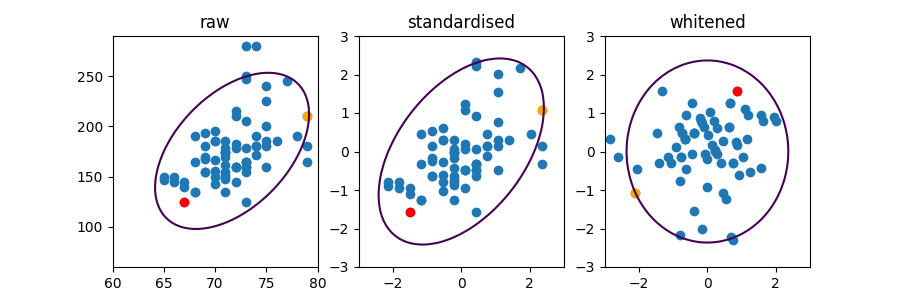
\includegraphics[width=\linewidth]{4-gaussian-models/48-whiten-stdise}
\end{figure}


\end{document}